%Version 3 October 2023
% See section 11 of the User Manual for version history
%
%%%%%%%%%%%%%%%%%%%%%%%%%%%%%%%%%%%%%%%%%%%%%%%%%%%%%%%%%%%%%%%%%%%%%%
%%                                                                 %%
%% Please do not use \input{...} to include other tex files.       %%
%% Submit your LaTeX manuscript as one .tex document.              %%
%%                                                                 %%
%% All additional figures and files should be attached             %%
%% separately and not embedded in the \TeX\ document itself.       %%
%%                                                                 %%
%%%%%%%%%%%%%%%%%%%%%%%%%%%%%%%%%%%%%%%%%%%%%%%%%%%%%%%%%%%%%%%%%%%%%

%%\documentclass[referee,sn-basic]{sn-jnl}% referee option is meant for double line spacing

%%=======================================================%%
%% to print line numbers in the margin use lineno option %%
%%=======================================================%%

%%\documentclass[lineno,sn-basic]{sn-jnl}% Basic Springer Nature Reference Style/Chemistry Reference Style

%%======================================================%%
%% to compile with pdflatex/xelatex use pdflatex option %%
%%======================================================%%

%%\documentclass[pdflatex,sn-basic]{sn-jnl}% Basic Springer Nature Reference Style/Chemistry Reference Style


%%Note: the following reference styles support Namedate and Numbered referencing. By default the style follows the most common style. To switch between the options you can add or remove �Numbered� in the optional parenthesis. 
%%The option is available for: sn-basic.bst, sn-vancouver.bst, sn-chicago.bst%  
 
%%\documentclass[sn-nature]{sn-jnl}% Style for submissions to Nature Portfolio journals
%%\documentclass[sn-basic]{sn-jnl}% Basic Springer Nature Reference Style/Chemistry Reference Style
\documentclass[sn-mathphys-num]{sn-jnl}% Math and Physical Sciences Numbered Reference Style 
%%\documentclass[sn-mathphys-ay]{sn-jnl}% Math and Physical Sciences Author Year Reference Style
%%\documentclass[sn-aps]{sn-jnl}% American Physical Society (APS) Reference Style``
%%\documentclass[sn-vancouver,Numbered]{sn-jnl}% Vancouver Reference Style
%%\documentclass[sn-apa]{sn-jnl}% APA Reference Style 
%%\documentclass[sn-chicago]{sn-jnl}% Chicago-based Humanities Reference Style

%%%% Standard Packages
%%<additional latex packages if required can be included here>

\usepackage{graphicx}%
\usepackage{multirow}%
\usepackage{amsmath,amssymb,amsfonts}%
\usepackage{amsthm}%
\usepackage{mathrsfs}%
\usepackage[title]{appendix}%
\usepackage{xcolor}%
\usepackage{textcomp}%
\usepackage{manyfoot}%
\usepackage{booktabs}%
\usepackage{algorithm}%
\usepackage{algorithmicx}%
\usepackage{algpseudocode}%
\usepackage{listings}%
%%%%

%%%%%=============================================================================%%%%
%%%%  Remarks: This template is provided to aid authors with the preparation
%%%%  of original research articles intended for submission to journals published 
%%%%  by Springer Nature. The guidance has been prepared in partnership with 
%%%%  production teams to conform to Springer Nature technical requirements. 
%%%%  Editorial and presentation requirements differ among journal portfolios and 
%%%%  research disciplines. You may find sections in this template are irrelevant 
%%%%  to your work and are empowered to omit any such section if allowed by the 
%%%%  journal you intend to submit to. The submission guidelines and policies 
%%%%  of the journal take precedence. A detailed User Manual is available in the 
%%%%  template package for technical guidance.
%%%%%=============================================================================%%%%

%% as per the requirement new theorem styles can be included as shown below
\theoremstyle{thmstyleone}%
\newtheorem{theorem}{Theorem}%  meant for continuous numbers
%%\newtheorem{theorem}{Theorem}[section]% meant for sectionwise numbers
%% optional argument [theorem] produces theorem numbering sequence instead of independent numbers for Proposition
\newtheorem{proposition}[theorem]{Proposition}% 
%%\newtheorem{proposition}{Proposition}% to get separate numbers for theorem and proposition etc.

\theoremstyle{thmstyletwo}%
\newtheorem{example}{Example}%
\newtheorem{remark}{Remark}%

\theoremstyle{thmstylethree}%
\newtheorem{definition}{Definition}%

\raggedbottom
%%\unnumbered% uncomment this for unnumbered level heads

\begin{document}

\title[Article Title]{Overpriced and Undersupplied: Density as a Measure of Demand in Large US Apartment Markets}

%%=============================================================%%
%% GivenName	-> \fnm{Joergen W.}
%% Particle	-> \spfx{van der} -> surname prefix
%% FamilyName	-> \sur{Ploeg}
%% Suffix	-> \sfx{IV}
%% \author*[1,2]{\fnm{Joergen W.} \spfx{van der} \sur{Ploeg} 
%%  \sfx{IV}}\email{iauthor@gmail.com}
%%=============================================================%%

\author*[1,2]{\fnm{First} \sur{Author}}\email{iauthor@gmail.com}

\author[2,3]{\fnm{Second} \sur{Author}}\email{iiauthor@gmail.com}
\equalcont{These authors contributed equally to this work.}

\author[1,2]{\fnm{Third} \sur{Author}}\email{iiiauthor@gmail.com}
\equalcont{These authors contributed equally to this work.}

\affil*[1]{\orgdiv{Department}, \orgname{Organization}, \orgaddress{\street{Street}, \city{City}, \postcode{100190}, \state{State}, \country{Country}}}

\affil[2]{\orgdiv{Department}, \orgname{Organization}, \orgaddress{\street{Street}, \city{City}, \postcode{10587}, \state{State}, \country{Country}}}

\affil[3]{\orgdiv{Department}, \orgname{Organization}, \orgaddress{\street{Street}, \city{City}, \postcode{610101}, \state{State}, \country{Country}}}

%%==================================%%
%% Sample for unstructured abstract %%
%%==================================%%

\abstract{We introduce an empirical measure of multifamily demand, based on density changes, and offer evidence of its segmenting and predictive power. Using this variable, we solve for the intersection of supply and demand curves each year for 20 years in each of the hundred largest MSAs in the United States. Over the 2,000 observations, we classified each sample as over or under-supplied and over-or-under-priced, based on the derived market-clearing rents and quantities, relative to observed rents and quantities. Grouping markets this way was highly predictive of their next-twelve-month rent growth, with the under-under group returning 2\% more annually than the over-over group. With this, we provide a better way to understand consumer housing demand; their indifference curve of space versus price; and the impact of supply shocks.}

%%================================%%
%% Sample for structured abstract %%
%%================================%%

% \abstract{\textbf{Purpose:} The abstract serves both as a general introduction to the topic and as a brief, non-technical summary of the main results and their implications. The abstract must not include subheadings (unless expressly permitted in the journal's Instructions to Authors), equations or citations. As a guide the abstract should not exceed 200 words. Most journals do not set a hard limit however authors are advised to check the author instructions for the journal they are submitting to.
% 
% \textbf{Methods:} The abstract serves both as a general introduction to the topic and as a brief, non-technical summary of the main results and their implications. The abstract must not include subheadings (unless expressly permitted in the journal's Instructions to Authors), equations or citations. As a guide the abstract should not exceed 200 words. Most journals do not set a hard limit however authors are advised to check the author instructions for the journal they are submitting to.
% 
% \textbf{Results:} The abstract serves both as a general introduction to the topic and as a brief, non-technical summary of the main results and their implications. The abstract must not include subheadings (unless expressly permitted in the journal's Instructions to Authors), equations or citations. As a guide the abstract should not exceed 200 words. Most journals do not set a hard limit however authors are advised to check the author instructions for the journal they are submitting to.
% 
% \textbf{Conclusion:} The abstract serves both as a general introduction to the topic and as a brief, non-technical summary of the main results and their implications. The abstract must not include subheadings (unless expressly permitted in the journal's Instructions to Authors), equations or citations. As a guide the abstract should not exceed 200 words. Most journals do not set a hard limit however authors are advised to check the author instructions for the journal they are submitting to.}

\keywords{keyword1, Keyword2, Keyword3, Keyword4}

%%\pacs[JEL Classification]{D8, H51}

%%\pacs[MSC Classification]{35A01, 65L10, 65L12, 65L20, 65L70}

\maketitle

\section{Introduction}\label{sec1}
\abstract{We introduce an empirical measure of multifamily demand, based on density changes, and offer evidence of its segmenting and predictive power. Using this variable, we solve for the intersection of supply and demand curves each year for 20 years in each of the hundred largest MSAs in the United States. Over the 2,000 observations, we classified each sample as over or under-supplied and over-or-under-priced, based on the derived market-clearing rents and quantities, relative to observed rents and quantities. Grouping markets this way was highly predictive of their next-twelve-month rent growth, with the under-under group returning 2\% more annually than the over-over group. With this, we provide a better way to understand consumer housing demand; their indifference curve of space versus price; and the impact of supply shocks.}  

   

The article investigates density as a measure of demand for multifamily real estate in the United States. With the level of home ownership at 65.6\% (US Census Bureau (1),2024), and the shifting of consumer preferences toward rental (Fannie Mae (2), 2024) the renter household will play a large role in the coming generations. The rent and its growth or decline remains then a highly relevant area of study, with the average consumer paying 31 percent* (USCB (3), 2024) of his or her income to rent. Some cite a lack of affordable housing as a culprit for rising rents [FIND SOURCE], but in the same breath, we hear caution for the wave of supply coming into multifamily housing [find news sources]. This seemingly contradictory sentiment belies a lack of a reliable measure of demand. In this article, we focus on a measure of demand outside of the traditional and self-referential variables of occupancy and absorption. We provide evidence that density--approximated by population over rental units--and its change indicates when a market is under or oversupplied and can be used to find the next year's rent growth.  

   

While most existing research on demand focuses on occupancy levels and absorption (Anenberg et al. (5), 2024; Phyrr et al. (6), 1999; Mueller (11), 1999), those two variables are capped at 100\%. A building cannot be 110\% occupied, nor can renters absorb more units than are produced. This system of measurement prohibits demand from ever exceeding supply. With this handicap, we can seek to find the relationships between supply and demand, but the literature may yield contradictory results (Ihlanfeldt et al. (7), 2014; Davidoff (8), 2015; Pennington (9), 2021; Molloy et al. (10), 2022). The problem matters because the intersection of supply and demand curves should suggest an equilibrium price, or a rent which renters, developers, and owners can use to gauge affordability, development profitability, and competitive rents. Some research aims to explain rent by examining occupancy levels at different stages of the physical market cycle (Mueller (11), 1999) or by analyzing how a city’s different characteristics interact with the various industries located there (Titman et al. (14), 2024).   

fill this out with references to some of the research you collected of how other studies look at rent growth.  

   

This research aims to introduce a demand variable that is not capped: density. If one had clear visibility into number-of-people per rental unit, then demand and utility curves could be derived. Under the assumptions that consumers prefer more space (Molloy et al. (10), 2022)**, then knowing the price at which a renter chose to live alone versus take a room mate would indicate the quantity of units demanded and the price at which those units would be demanded. Prior work has explored density, and while density appears to be a net amenity, part of the rent increase associated with higher density may be attributable to the higher cost of providing space. For some renters, increased density can translate to desirable urban living spaces, surrounded by jobs and amenities while for others, it can result in overcrowding and reduced quality of life. Policy induced densification may involve a net cost to renters and first-time homebuyers (Ahlfeldt et al. (12), 2019; Albouy et al. (13), 2015). 

   

But that does not fully address the question. None of the previous studies define density as population divided by rental units, but instead as population divided by area or as units divided by area. Not all parts of a city are residential and to that end, not all parts are even habitable, due to geographic or other restrictions. These density metrics are not effective in capturing the level of supply relative to the population in an MSA.  

   

Our main contribution is to provide evidence of the use of density as a measure of demand. Other work has explored demand from an agglomeration point-of-view, modeling the benefits of agglomeration externalities, and exploring how agglomeration affects rents in urban areas (Titman et al. (14), 2024; Liu et al. (15), 2018). And that nods to the cyclical unique nature of real estate--where more density can make a more valuable commodity that can in turn produce more density. A paradigm where a renter is willing to pay more for less space in Manhattan, when she could pay less for more space in Houston. MSA-level density and its year-over-year change reveals a proxy of demand which indicates whether rents will grow in the near-term. We call this metric implied demand and show that it provides evidence of over or undersupply and over or underpricing.  

   

Our article also speaks to the broader debate of rent affordability, the need for more housing, and the local differences inherent in such discussions. From the owner/developer standpoint, a more useful measure of demand could dampen real estate development cycles, which often result in unexpectedly depressed rents. From the renter's standpoint, a more useful demand metric can help identify locations where rent is likely to grow, maintain, or decrease, relative to inflation.  

   

Focusing on a panel of the 100 largest metropolitan statistical areas (MSA), their population, rental unit count, and change in rent, we estimate implied demand of each MSA at each of 10 years from 2013 to 2023. We plot this against rent to derive a demand curve. We then take the observed supply growth of each MSA and plot it against rent to derive a supply curve. The intersection of those two curves is the derived point of supply and rent equilibrium. Comparing a market's actual rent to the market's derived rent suggests over or underpricing. Comparing a market's actual supply growth to the market's derived supply growth provides evidence of over or undersupply. We show that by segmenting markets as over or undersupplied and over or underpriced each year, we can effectively forecast the market's next-year rent growth.  
  

In the Data section we describe the data we used and analyze its properties. The subsequent section (Experiment) illustrates statistical tests performed to evaluate the validity of the classifications. And the final section discusses the results and concludes. 
 
\section{Existing Measures of Demand}
Occupancy and vacancy and absorption are sloped the wrong way and or 
are capped at 1
First, we would expect the relationship between quantity and price to be inversely related such that the renter would prefer 1000 square feet to 500 square feet if the price were the same. Conversely,  the renter will settle for 250 square feet (likely sharing the unit) if prices are too high. 
For example, New York City in a given year may have a derived rent and quantity suggesting that 10\% more stock is demanded at 5\% higher prices. We compare that to the top-100 markets' values and see that the median derived stock is  but we may observe that nationally only 2\% more stock was delivered in the given year, and rents rose only by 3\%. This would be a situation of under-supply and under-pricing, and we would expect that disequilibrium to manifest in the future through rent growth. Because rent growth is not subject to sticky pricing, it should reflect disequilibrium more robustly than supply growth.

\section{Finding Demand through Density}
Density has a network-affect in real estate that is not common to other real assets. A telephone network would be useless if it had only one customer: whom would she call? But if ten people are on the network, the value of the network increases. So too in cities where agglomeration econonmics take effect. This phenomenon makes it so both the employer and employee are better off when there are many other firms in a short distance. The employee has higher employment security knowing he can shift firms if needed. The employer has a larger workforce available so he can scale up if needed. [find a reference]. Socially, the dense city offers ease of connection and more options of recreation. For these reasons, density, or a lack of space, is a worthwile tradeoff. Economically however it means that a renter will pay more for less space.

This occurs both at the unit level and at the city level. A renter may opt out of a 1000-square-foot unit in a suburb for a 500-square-foot unit in a city. Or, she may opt share a 1000 sqare-foot unit with a roomate. When viewed in aggregate, the population of a city and its total rental units provides a valiable quotient we call \textit{rental density index} or RDI. The RDI can be understood as the theoretical density an MSA would incur to house its entire population in rental units. It is not meant as a goal or to have intuitive readthrough but to serve as a reference point for the utility curve of a city's residents. 
The RDI contains latent information regarding homeownership, cohabitation preferences, and family size. The RDI moves slowly over time and is densely concentrated across MSAs. The mean RDI decreases in sync with the observed decrease in people-per-household in the US [find reference].

\begin{figure}[H]
	\centering
	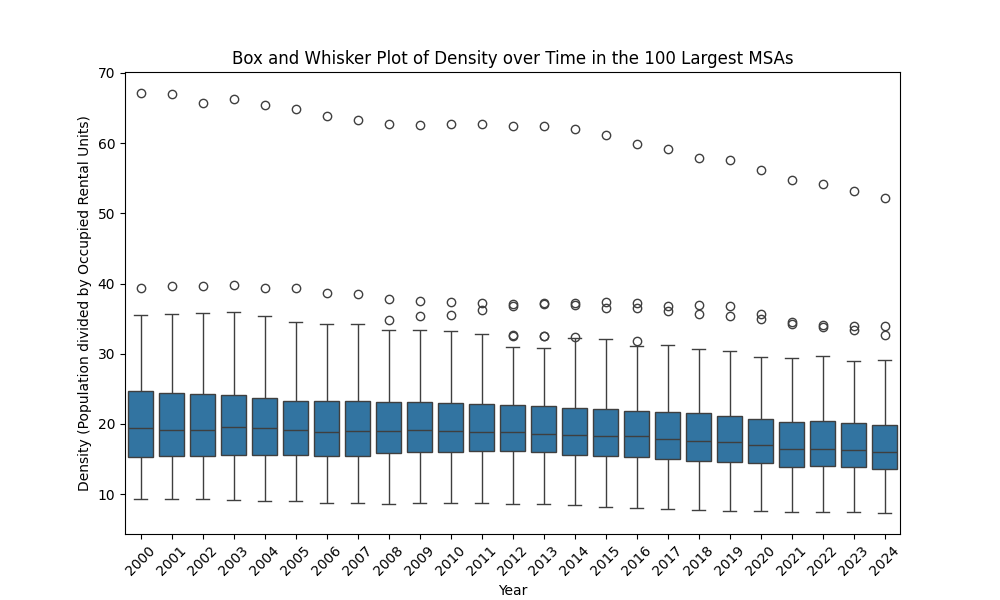
\includegraphics[width=0.9\textwidth]{"C:/Users/mlarriva/Documents/GitHub/demand_density/Figs/box_whisker_density_time.png"}
	\caption{This is a widefig. This is an example of long caption this is an example of long caption  this is an example of long caption this is an example of long caption}\label{fig1}
\end{figure}

\begin{figure}[H]
	\centering
	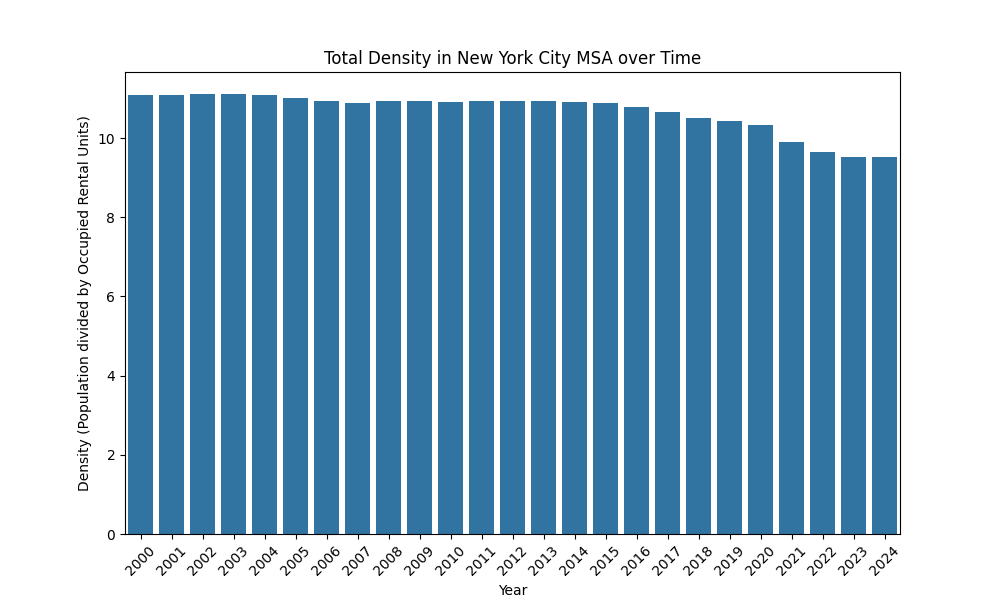
\includegraphics[width=0.9\textwidth]{"C:/Users/mlarriva/Documents/GitHub/demand_density/Figs/bar_total_density_year.png"}
	\caption{This is a widefig. This is an example of long caption this is an example of long caption  this is an example of long caption this is an example of long caption}\label{fig2}
\end{figure}

While the RDI indicates preferences across time and region, the change in the rental density index or $\Delta\text{RDI}$ is the focus of this work. The year-over-year change in the RDI is an information-rich variable both alone, in comparison to other MSAs, and in conjunction with rent changes. When combined with the rent per-square-foot the $\Delta\text{RDI}$ indicates when renters would prefer to cohabitate rather than absorb more space. It suggests a level at which more units would be demanded, and it provides insight into the level at which over and undersupply occur. 
Summary metrics follow.

\begin{figure}[H]
	\centering
	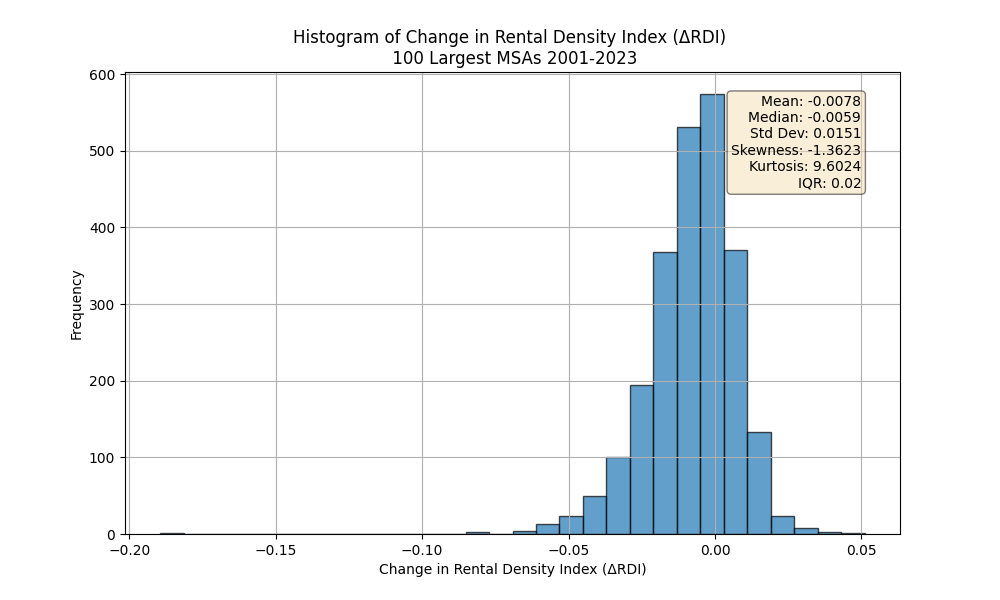
\includegraphics[width=0.9\textwidth]{"C:/Users/mlarriva/Documents/GitHub/demand_density/Figs/hist_deltardi.png"}
	\caption{This is a widefig. This is an example of long caption this is an example of long caption  this is an example of long caption this is an example of long caption}\label{fig3}
\end{figure}

Nationally, the relationship between $\Delta\text{RDI}$ and rent growth is inverse: rent growth decreases when renters cohabitate; it increases when renters demand their own units and absorb limited stock. This creates a downward sloping demand curve which we can use to find the intersection with the supply curve. 

\begin{figure}[H]
	\centering
	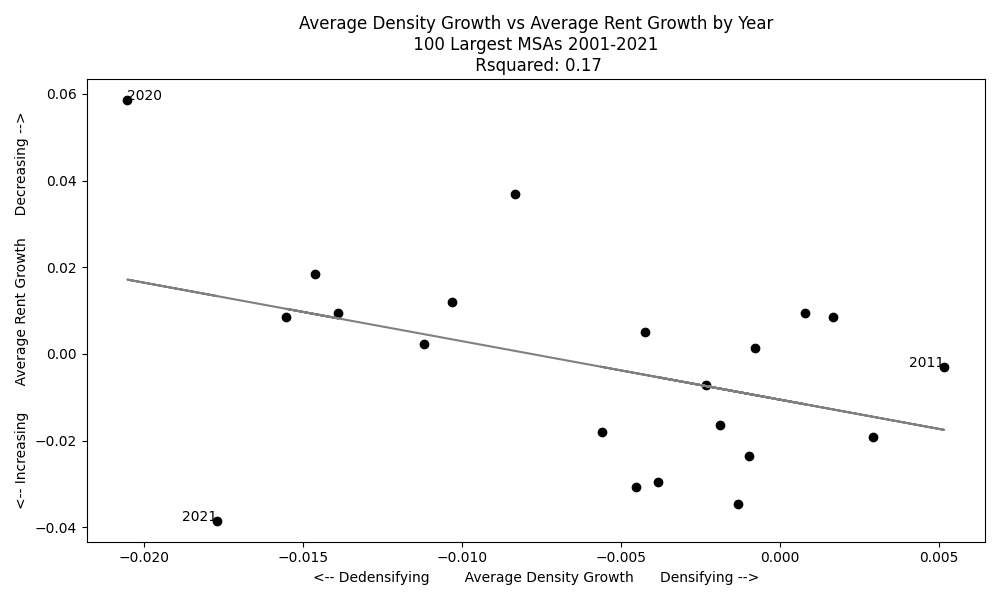
\includegraphics[width=0.9\textwidth]{"C:/Users/mlarriva/Documents/GitHub/demand_density/Figs/national_example.png"}
	\caption{This is a widefig. This is an example of long caption this is an example of long caption  this is an example of long caption this is an example of long caption}\label{fig4}
\end{figure}


\section{Empirical Evidence}\label{sec2}
Our objective is to analyze $\Delta\text{RDI}$ as a meaningful measure of demand. We do so by creating a demand curve for each MSA, for each year, plotting the trailing-10 years of $\Delta\text{RDI}$ against real rent per square foot. We intersect this line with the supply line. The supply line is defined as new supply as a percent of existing stock versus the real rent per square foot. The intersection of the supply and our demand curve produces the derived quantity (q*) and derived price (p*). These derived values (p*,q*) may be higher or lower than the actual market price and supply values (p,q). If the derived price (p*) is greater than (less than) p, then we say a market is underpriced (overpriced). If the derived quantity q* is greater than (less than) the observed quantity q then we say a market is undersupplied (oversupplied).

In any point in time, a market can then be in one of four states: overpriced undersupplied; overpriced oversupplied; underpriced undersupplied; underpriced oversupplied. We can call an overpriced and undersupplied market a landlord-favorable market. Conversely a market that is underpriced and oversupplied would be a renter-favorable market. Other combinations are neither renter nor landlord-favorable. We would expect lanlord-favorable markets to see higher rent growth the following year, as inventory is slow-moving prices will adjust up as landlords see there are few alternatives for new or renewing renters. Conversely, we would expect a renter-favorable market to see lower rent growth the following year, as landlords lower rents to incentivize renters to fill their vacant units. 

\begin{table}[h!]
\centering
\begin{tabular}{cc|c|c|}
\multicolumn{2}{c}{} & \multicolumn{2}{c}{\textbf{Pricing}} \\
\multicolumn{2}{c}{} & \textbf{Overpriced} & \textbf{Underpriced} \\
\cmidrule{3-4}
\multirow{2}{*}{\textbf{Supply}} & \textbf{Oversupplied} & Neutral & Renter Friendly \\\cmidrule{2-4}
 & \textbf{Undersupplied} & Landlord Friendly & Neutral \\
\bottomrule
\end{tabular}
\caption{Hypothesized NTM real rent-growth outcomes based on mispricing and mis-supplying}
\end{table}


\begin{algorithm}
	\caption{Segment Markets Into Over/Underpriced and Over/Undersupplied}\label{alg:market_segmentation}
	\begin{algorithmic}[1]
		\For{each year $y$ from [2010 to 2022]}
		    \For{each market $m$ in the top 100 markets}
		        \State Using the trailing 10 years' data...
		        \State $demandcurve$ = linear regression of  $\Delta\text{RDI}$  vs price-psf
		        \State $supplycurve$ = linear regression of supply growth vs price-psf
		        \State $(q^*, p^*)$ = Intersection of $supplycurve$ and $demandcurve$
		        \State $(q, p)$ = market's actual supply and price-per-square-foot in year $y$
		        \If{$q^* > q$} 
		            \If{$p^* > p$}
		                \State Assign market $m$ in year $y$ to Group \textbf{OversuppliedUnderpriced}
		            \Else
		                \State Assign market $m$ in year $y$ to Group \textbf{OversuppliedOverpriced}
		            \EndIf
		        \Else
		            \If{$p^* > p$}
		                \State Assign market $m$ in year $y$ to Group \textbf{UndersuppliedUnderpriced}
		            \Else
		                \State Assign market $m$ in year $y$ to Group \textbf{UndersuppliedOverpriced}
		            \EndIf
		        \EndIf
		    \EndFor
		\EndFor
	\end{algorithmic}
\end{algorithm}


As an example:




\section{Results}\label{sec2}

Sample body text. Sample body text. Sample body text. Sample body text. Sample body text. Sample body text. Sample body text. Sample body text.

\section{This is an example for first level head---section head}\label{sec3}

\subsection{This is an example for second level head---subsection head}\label{subsec2}

\subsubsection{This is an example for third level head---subsubsection head}\label{subsubsec2}

Sample body text. Sample body text. Sample body text. Sample body text. Sample body text. Sample body text. Sample body text. Sample body text.

\section{Equations}\label{sec4}

Equations in \LaTeX\ can either be inline or on-a-line by itself (``display equations''). For
inline equations use the \verb+$...$+ commands. E.g.: The equation
$H\psi = E \psi$ is written via the command \verb+$H \psi = E \psi$+.

For display equations (with auto generated equation numbers)
one can use the equation or align environments:
\begin{equation}
    \|\tilde{X}(k)\|^2 \leq\frac{\sum\limits_{i=1}^{p}\left\|\tilde{Y}_i(k)\right\|^2+\sum\limits_{j=1}^{q}\left\|\tilde{Z}_j(k)\right\|^2 }{p+q}.\label{eq1}
\end{equation}
where,
\begin{align}
    D_\mu        & =  \partial_\mu - ig \frac{\lambda^a}{2} A^a_\mu \nonumber                            \\
    F^a_{\mu\nu} & = \partial_\mu A^a_\nu - \partial_\nu A^a_\mu + g f^{abc} A^b_\mu A^a_\nu \label{eq2}
\end{align}
Notice the use of \verb+\nonumber+ in the align environment at the end
of each line, except the last, so as not to produce equation numbers on
lines where no equation numbers are required. The \verb+\label{}+ command
should only be used at the last line of an align environment where
\verb+\nonumber+ is not used.
\begin{equation}
    Y_\infty = \left( \frac{m}{\textrm{GeV}} \right)^{-3}
    \left[ 1 + \frac{3 \ln(m/\textrm{GeV})}{15}
        + \frac{\ln(c_2/5)}{15} \right]
\end{equation}
The class file also supports the use of \verb+\mathbb{}+, \verb+\mathscr{}+ and
\verb+\mathcal{}+ commands. As such \verb+\mathbb{R}+, \verb+\mathscr{R}+
and \verb+\mathcal{R}+ produces $\mathbb{R}$, $\mathscr{R}$ and $\mathcal{R}$
respectively (refer Subsubsection~\ref{subsubsec2}).

\section{Tables}\label{sec5}

Tables can be inserted via the normal table and tabular environment. To put
footnotes inside tables you should use \verb+\footnotetext[]{...}+ tag.
The footnote appears just below the table itself (refer Tables~\ref{tab1} and \ref{tab2}).
For the corresponding footnotemark use \verb+\footnotemark[...]+

\begin{table}[h]
    \caption{Caption text}\label{tab1}%
    \begin{tabular}{@{}llll@{}}
        \toprule
        Column 1 & Column 2 & Column 3               & Column 4               \\
        \midrule
        row 1    & data 1   & data 2                 & data 3                 \\
        row 2    & data 4   & data 5\footnotemark[1] & data 6                 \\
        row 3    & data 7   & data 8                 & data 9\footnotemark[2] \\
        \botrule
    \end{tabular}
    \footnotetext{Source: This is an example of table footnote. This is an example of table footnote.}
    \footnotetext[1]{Example for a first table footnote. This is an example of table footnote.}
    \footnotetext[2]{Example for a second table footnote. This is an example of table footnote.}
\end{table}

\noindent
The input format for the above table is as follows:

%%=============================================%%
%% For presentation purpose, we have included  %%
%% \bigskip command. Please ignore this.       %%
%%=============================================%%
\bigskip
\begin{verbatim}
\begin{table}[<placement-specifier>]
\caption{<table-caption>}\label{<table-label>}%
\begin{tabular}{@{}llll@{}}
\toprule
Column 1 & Column 2 & Column 3 & Column 4\\
\midrule
row 1 & data 1 & data 2	 & data 3 \\
row 2 & data 4 & data 5\footnotemark[1] & data 6 \\
row 3 & data 7 & data 8	 & data 9\footnotemark[2]\\
\botrule
\end{tabular}
\footnotetext{Source: This is an example of table footnote. 
This is an example of table footnote.}
\footnotetext[1]{Example for a first table footnote.
This is an example of table footnote.}
\footnotetext[2]{Example for a second table footnote. 
This is an example of table footnote.}
\end{table}
\end{verbatim}
\bigskip
%%=============================================%%
%% For presentation purpose, we have included  %%
%% \bigskip command. Please ignore this.       %%
%%=============================================%%

\begin{table}[h]
    \caption{Example of a lengthy table which is set to full textwidth}\label{tab2}
    \begin{tabular*}{\textwidth}{@{\extracolsep\fill}lcccccc}
        \toprule%
        & \multicolumn{3}{@{}c@{}}{Element 1\footnotemark[1]} & \multicolumn{3}{@{}c@{}}{Element 2\footnotemark[2]} \\\cmidrule{2-4}\cmidrule{5-7}%
        Project & Energy & $\sigma_{calc}$ & $\sigma_{expt}$ & Energy & $\sigma_{calc}$ & $\sigma_{expt}$ \\
        \midrule
        Element 3  & 990 A & 1168 & $1547\pm12$ & 780 A & 1166 & $1239\pm100$\\
        Element 4  & 500 A & 961  & $922\pm10$  & 900 A & 1268 & $1092\pm40$\\
        \botrule
    \end{tabular*}
    \footnotetext{Note: This is an example of table footnote. This is an example of table footnote this is an example of table footnote this is an example of~table footnote this is an example of table footnote.}
    \footnotetext[1]{Example for a first table footnote.}
    \footnotetext[2]{Example for a second table footnote.}
\end{table}

In case of double column layout, tables which do not fit in single column width should be set to full text width. For this, you need to use \verb+\begin{table*}+ \verb+...+ \verb+\end{table*}+ instead of \verb+\begin{table}+ \verb+...+ \verb+\end{table}+ environment. Lengthy tables which do not fit in textwidth should be set as rotated table. For this, you need to use \verb+\begin{sidewaystable}+ \verb+...+ \verb+\end{sidewaystable}+ instead of \verb+\begin{table*}+ \verb+...+ \verb+\end{table*}+ environment. This environment puts tables rotated to single column width. For tables rotated to double column width, use \verb+\begin{sidewaystable*}+ \verb+...+ \verb+\end{sidewaystable*}+.

\begin{sidewaystable}
    \caption{Tables which are too long to fit, should be written using the ``sidewaystable'' environment as shown here}\label{tab3}
    \begin{tabular*}{\textheight}{@{\extracolsep\fill}lcccccc}
        \toprule%
        & \multicolumn{3}{@{}c@{}}{Element 1\footnotemark[1]}& \multicolumn{3}{@{}c@{}}{Element\footnotemark[2]} \\\cmidrule{2-4}\cmidrule{5-7}%
        Projectile & Energy	& $\sigma_{calc}$ & $\sigma_{expt}$ & Energy & $\sigma_{calc}$ & $\sigma_{expt}$ \\
        \midrule
        Element 3 & 990 A & 1168 & $1547\pm12$ & 780 A & 1166 & $1239\pm100$ \\
        Element 4 & 500 A & 961  & $922\pm10$  & 900 A & 1268 & $1092\pm40$ \\
        Element 5 & 990 A & 1168 & $1547\pm12$ & 780 A & 1166 & $1239\pm100$ \\
        Element 6 & 500 A & 961  & $922\pm10$  & 900 A & 1268 & $1092\pm40$ \\
        \botrule
    \end{tabular*}
    \footnotetext{Note: This is an example of table footnote this is an example of table footnote this is an example of table footnote this is an example of~table footnote this is an example of table footnote.}
    \footnotetext[1]{This is an example of table footnote.}
\end{sidewaystable}

\section{Figures}\label{sec6}

As per the \LaTeX\ standards you need to use eps images for \LaTeX\ compilation and \verb+pdf/jpg/png+ images for \verb+PDFLaTeX+ compilation. This is one of the major difference between \LaTeX\ and \verb+PDFLaTeX+. Each image should be from a single input .eps/vector image file. Avoid using subfigures. The command for inserting images for \LaTeX\ and \verb+PDFLaTeX+ can be generalized. The package used to insert images in \verb+LaTeX/PDFLaTeX+ is the graphicx package. Figures can be inserted via the normal figure environment as shown in the below example:

%%=============================================%%
%% For presentation purpose, we have included  %%
%% \bigskip command. Please ignore this.       %%
%%=============================================%%
\bigskip
\begin{verbatim}
\begin{figure}[<placement-specifier>]
\centering
\includegraphics{<eps-file>}
\caption{<figure-caption>}\label{<figure-label>}
\end{figure}
\end{verbatim}
\bigskip
%%=============================================%%
%% For presentation purpose, we have included  %%
%% \bigskip command. Please ignore this.       %%
%%=============================================%%

\begin{figure}[h]
    \centering
    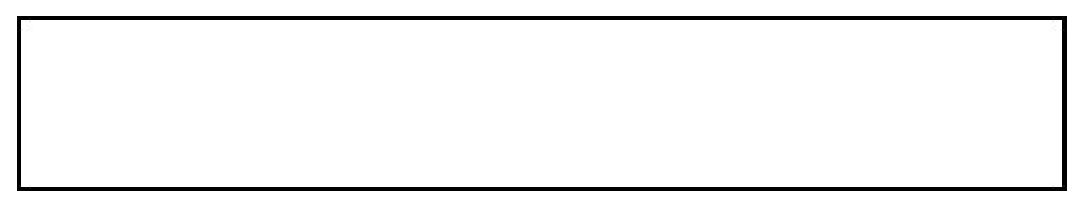
\includegraphics[width=0.9\textwidth]{fig.eps}
    \caption{This is a widefig. This is an example of long caption this is an example of long caption  this is an example of long caption this is an example of long caption}\label{fig1}
\end{figure}

In case of double column layout, the above format puts figure captions/images to single column width. To get spanned images, we need to provide \verb+\begin{figure*}+ \verb+...+ \verb+\end{figure*}+.

For sample purpose, we have included the width of images in the optional argument of \verb+\includegraphics+ tag. Please ignore this.

\section{Algorithms, Program codes and Listings}\label{sec7}

Packages \verb+algorithm+, \verb+algorithmicx+ and \verb+algpseudocode+ are used for setting algorithms in \LaTeX\ using the format:

%%=============================================%%
%% For presentation purpose, we have included  %%
%% \bigskip command. Please ignore this.       %%
%%=============================================%%
\bigskip
\begin{verbatim}
\begin{algorithm}
\caption{<alg-caption>}\label{<alg-label>}
\begin{algorithmic}[1]
. . .
\end{algorithmic}
\end{algorithm}
\end{verbatim}
\bigskip
%%=============================================%%
%% For presentation purpose, we have included  %%
%% \bigskip command. Please ignore this.       %%
%%=============================================%%

You may refer above listed package documentations for more details before setting \verb+algorithm+ environment. For program codes, the ``verbatim'' package is required and the command to be used is \verb+\begin{verbatim}+ \verb+...+ \verb+\end{verbatim}+.

Similarly, for \verb+listings+, use the \verb+listings+ package. \verb+\begin{lstlisting}+ \verb+...+ \verb+\end{lstlisting}+ is used to set environments similar to \verb+verbatim+ environment. Refer to the \verb+lstlisting+ package documentation for more details.

A fast exponentiation procedure:

\lstset{texcl=true,basicstyle=\small\sf,commentstyle=\small\rm,mathescape=true,escapeinside={(*}{*)}}
\begin{lstlisting}
begin
  for $i:=1$ to $10$ step $1$ do
      expt($2,i$);  
      newline() od                (*\textrm{Comments will be set flush to the right margin}*)
where
proc expt($x,n$) $\equiv$
  $z:=1$;
  do if $n=0$ then exit fi;
     do if odd($n$) then exit fi;                 
        comment: (*\textrm{This is a comment statement;}*)
        $n:=n/2$; $x:=x*x$ od;
     { $n>0$ };
     $n:=n-1$; $z:=z*x$ od;
  print($z$). 
end
\end{lstlisting}

\begin{algorithm}
    \caption{Calculate $y = x^n$}\label{algo1}
    \begin{algorithmic}[1]
        \Require $n \geq 0 \vee x \neq 0$
        \Ensure $y = x^n$
        \State $y \Leftarrow 1$
        \If{$n < 0$}\label{algln2}
        \State $X \Leftarrow 1 / x$
        \State $N \Leftarrow -n$
        \Else
        \State $X \Leftarrow x$
        \State $N \Leftarrow n$
        \EndIf
        \While{$N \neq 0$}
        \If{$N$ is even}
        \State $X \Leftarrow X \times X$
        \State $N \Leftarrow N / 2$
        \Else[$N$ is odd]
        \State $y \Leftarrow y \times X$
        \State $N \Leftarrow N - 1$
        \EndIf
        \EndWhile
    \end{algorithmic}
\end{algorithm}

%%=============================================%%
%% For presentation purpose, we have included  %%
%% \bigskip command. Please ignore this.       %%
%%=============================================%%
\bigskip
\begin{minipage}{\hsize}%
    \lstset{frame=single,framexleftmargin=-1pt,framexrightmargin=-17pt,framesep=12pt,linewidth=0.98\textwidth,language=pascal}% Set your language (you can change the language for each code-block optionally)
    %%% Start your code-block
    \begin{lstlisting}
for i:=maxint to 0 do
begin
{ do nothing }
end;
Write('Case insensitive ');
Write('Pascal keywords.');
\end{lstlisting}
\end{minipage}

\section{Cross referencing}\label{sec8}

Environments such as figure, table, equation and align can have a label
declared via the \verb+\label{#label}+ command. For figures and table
environments use the \verb+\label{}+ command inside or just
below the \verb+\caption{}+ command. You can then use the
\verb+\ref{#label}+ command to cross-reference them. As an example, consider
the label declared for Figure~\ref{fig1} which is
\verb+\label{fig1}+. To cross-reference it, use the command
\verb+Figure \ref{fig1}+, for which it comes up as
``Figure~\ref{fig1}''.

To reference line numbers in an algorithm, consider the label declared for the line number 2 of Algorithm~\ref{algo1} is \verb+\label{algln2}+. To cross-reference it, use the command \verb+\ref{algln2}+ for which it comes up as line~\ref{algln2} of Algorithm~\ref{algo1}.

\subsection{Details on reference citations}\label{subsec7}

Standard \LaTeX\ permits only numerical citations. To support both numerical and author-year citations this template uses \verb+natbib+ \LaTeX\ package. For style guidance please refer to the template user manual.

Here is an example for \verb+\cite{...}+: \cite{bib1}. Another example for \verb+\citep{...}+: \citep{bib2}. For author-year citation mode, \verb+\cite{...}+ prints Jones et al. (1990) and \verb+\citep{...}+ prints (Jones et al., 1990).

All cited bib entries are printed at the end of this article: \cite{bib3}, \cite{bib4}, \cite{bib5}, \cite{bib6}, \cite{bib7}, \cite{bib8}, \cite{bib9}, \cite{bib10}, \cite{bib11}, \cite{bib12} and \cite{bib13}.


\section{Examples for theorem like environments}\label{sec10}

For theorem like environments, we require \verb+amsthm+ package. There are three types of predefined theorem styles exists---\verb+thmstyleone+, \verb+thmstyletwo+ and \verb+thmstylethree+

%%=============================================%%
%% For presentation purpose, we have included  %%
%% \bigskip command. Please ignore this.       %%
%%=============================================%%
\bigskip
\begin{tabular}{|l|p{19pc}|}
    \hline
    \verb+thmstyleone+   & Numbered, theorem head in bold font and theorem text in italic style  \\\hline
    \verb+thmstyletwo+   & Numbered, theorem head in roman font and theorem text in italic style \\\hline
    \verb+thmstylethree+ & Numbered, theorem head in bold font and theorem text in roman style   \\\hline
\end{tabular}
\bigskip
%%=============================================%%
%% For presentation purpose, we have included  %%
%% \bigskip command. Please ignore this.       %%
%%=============================================%%

For mathematics journals, theorem styles can be included as shown in the following examples:

\begin{theorem}[Theorem subhead]\label{thm1}
    Example theorem text. Example theorem text. Example theorem text. Example theorem text. Example theorem text.
    Example theorem text. Example theorem text. Example theorem text. Example theorem text. Example theorem text.
    Example theorem text.
\end{theorem}

Sample body text. Sample body text. Sample body text. Sample body text. Sample body text. Sample body text. Sample body text. Sample body text.

\begin{proposition}
    Example proposition text. Example proposition text. Example proposition text. Example proposition text. Example proposition text.
    Example proposition text. Example proposition text. Example proposition text. Example proposition text. Example proposition text.
\end{proposition}

Sample body text. Sample body text. Sample body text. Sample body text. Sample body text. Sample body text. Sample body text. Sample body text.

\begin{example}
    Phasellus adipiscing semper elit. Proin fermentum massa
    ac quam. Sed diam turpis, molestie vitae, placerat a, molestie nec, leo. Maecenas lacinia. Nam ipsum ligula, eleifend
    at, accumsan nec, suscipit a, ipsum. Morbi blandit ligula feugiat magna. Nunc eleifend consequat lorem.
\end{example}

Sample body text. Sample body text. Sample body text. Sample body text. Sample body text. Sample body text. Sample body text. Sample body text.

\begin{remark}
    Phasellus adipiscing semper elit. Proin fermentum massa
    ac quam. Sed diam turpis, molestie vitae, placerat a, molestie nec, leo. Maecenas lacinia. Nam ipsum ligula, eleifend
    at, accumsan nec, suscipit a, ipsum. Morbi blandit ligula feugiat magna. Nunc eleifend consequat lorem.
\end{remark}

Sample body text. Sample body text. Sample body text. Sample body text. Sample body text. Sample body text. Sample body text. Sample body text.

\begin{definition}[Definition sub head]
    Example definition text. Example definition text. Example definition text. Example definition text. Example definition text. Example definition text. Example definition text. Example definition text.
\end{definition}

Additionally a predefined ``proof'' environment is available: \verb+\begin{proof}+ \verb+...+ \verb+\end{proof}+. This prints a ``Proof'' head in italic font style and the ``body text'' in roman font style with an open square at the end of each proof environment.

\begin{proof}
    Example for proof text. Example for proof text. Example for proof text. Example for proof text. Example for proof text. Example for proof text. Example for proof text. Example for proof text. Example for proof text. Example for proof text.
\end{proof}

Sample body text. Sample body text. Sample body text. Sample body text. Sample body text. Sample body text. Sample body text. Sample body text.

\begin{proof}[Proof of Theorem~{\upshape\ref{thm1}}]
    Example for proof text. Example for proof text. Example for proof text. Example for proof text. Example for proof text. Example for proof text. Example for proof text. Example for proof text. Example for proof text. Example for proof text.
\end{proof}

\noindent
For a quote environment, use \verb+\begin{quote}...\end{quote}+
\begin{quote}
    Quoted text example. Aliquam porttitor quam a lacus. Praesent vel arcu ut tortor cursus volutpat. In vitae pede quis diam bibendum placerat. Fusce elementum
    convallis neque. Sed dolor orci, scelerisque ac, dapibus nec, ultricies ut, mi. Duis nec dui quis leo sagittis commodo.
\end{quote}

Sample body text. Sample body text. Sample body text. Sample body text. Sample body text (refer Figure~\ref{fig1}). Sample body text. Sample body text. Sample body text (refer Table~\ref{tab3}).

\section{Methods}\label{sec11}

Topical subheadings are allowed. Authors must ensure that their Methods section includes adequate experimental and characterization data necessary for others in the field to reproduce their work. Authors are encouraged to include RIIDs where appropriate.

\textbf{Ethical approval declarations} (only required where applicable) Any article reporting experiment/s carried out on (i)~live vertebrate (or higher invertebrates), (ii)~humans or (iii)~human samples must include an unambiguous statement within the methods section that meets the following requirements:

\begin{enumerate}[1.]
    \item Approval: a statement which confirms that all experimental protocols were approved by a named institutional and/or licensing committee. Please identify the approving body in the methods section

    \item Accordance: a statement explicitly saying that the methods were carried out in accordance with the relevant guidelines and regulations

    \item Informed consent (for experiments involving humans or human tissue samples): include a statement confirming that informed consent was obtained from all participants and/or their legal guardian/s
\end{enumerate}

If your manuscript includes potentially identifying patient/participant information, or if it describes human transplantation research, or if it reports results of a clinical trial then  additional information will be required. Please visit (\url{https://www.nature.com/nature-research/editorial-policies}) for Nature Portfolio journals, (\url{https://www.springer.com/gp/authors-editors/journal-author/journal-author-helpdesk/publishing-ethics/14214}) for Springer Nature journals, or (\url{https://www.biomedcentral.com/getpublished/editorial-policies\#ethics+and+consent}) for BMC.

\section{Discussion}\label{sec12}

Discussions should be brief and focused. In some disciplines use of Discussion or `Conclusion' is interchangeable. It is not mandatory to use both. Some journals prefer a section `Results and Discussion' followed by a section `Conclusion'. Please refer to Journal-level guidance for any specific requirements.

\section{Conclusion}\label{sec13}

Conclusions may be used to restate your hypothesis or research question, restate your major findings, explain the relevance and the added value of your work, highlight any limitations of your study, describe future directions for research and recommendations.

In some disciplines use of Discussion or 'Conclusion' is interchangeable. It is not mandatory to use both. Please refer to Journal-level guidance for any specific requirements.

\backmatter

\bmhead{Supplementary information}

If your article has accompanying supplementary file/s please state so here.

Authors reporting data from electrophoretic gels and blots should supply the full unprocessed scans for key as part of their Supplementary information. This may be requested by the editorial team/s if it is missing.

Please refer to Journal-level guidance for any specific requirements.

\bmhead{Acknowledgements}

Acknowledgements are not compulsory. Where included they should be brief. Grant or contribution numbers may be acknowledged.

Please refer to Journal-level guidance for any specific requirements.

\section*{Declarations}

Some journals require declarations to be submitted in a standardised format. Please check the Instructions for Authors of the journal to which you are submitting to see if you need to complete this section. If yes, your manuscript must contain the following sections under the heading `Declarations':

\begin{itemize}
    \item Funding
    \item Conflict of interest/Competing interests (check journal-specific guidelines for which heading to use)
    \item Ethics approval and consent to participate
    \item Consent for publication
    \item Data availability
    \item Materials availability
    \item Code availability
    \item Author contribution
\end{itemize}

\noindent
If any of the sections are not relevant to your manuscript, please include the heading and write `Not applicable' for that section.

%%===================================================%%
%% For presentation purpose, we have included        %%
%% \bigskip command. Please ignore this.             %%
%%===================================================%%
\bigskip
\begin{flushleft}%
    Editorial Policies for:

    \bigskip\noindent
    Springer journals and proceedings: \url{https://www.springer.com/gp/editorial-policies}

    \bigskip\noindent
    Nature Portfolio journals: \url{https://www.nature.com/nature-research/editorial-policies}

    \bigskip\noindent
    \textit{Scientific Reports}: \url{https://www.nature.com/srep/journal-policies/editorial-policies}

    \bigskip\noindent
    BMC journals: \url{https://www.biomedcentral.com/getpublished/editorial-policies}
\end{flushleft}

\begin{appendices}

    \section{Section title of first appendix}\label{secA1}

    An appendix contains supplementary information that is not an essential part of the text itself but which may be helpful in providing a more comprehensive understanding of the research problem or it is information that is too cumbersome to be included in the body of the paper.

    %%=============================================%%
    %% For submissions to Nature Portfolio Journals %%
    %% please use the heading ``Extended Data''.   %%
    %%=============================================%%

    %%=============================================================%%
    %% Sample for another appendix section			       %%
    %%=============================================================%%

    %% \section{Example of another appendix section}\label{secA2}%
    %% Appendices may be used for helpful, supporting or essential material that would otherwise 
    %% clutter, break up or be distracting to the text. Appendices can consist of sections, figures, 
    %% tables and equations etc.

\end{appendices}

%%===========================================================================================%%
%% If you are submitting to one of the Nature Portfolio journals, using the eJP submission   %%
%% system, please include the references within the manuscript file itself. You may do this  %%
%% by copying the reference list from your .bbl file, paste it into the main manuscript .tex %%
%% file, and delete the associated \verb+\bibliography+ commands.                            %%
%%===========================================================================================%%

\bibliography{sn-bibliography}% common bib file
%% if required, the content of .bbl file can be included here once bbl is generated
%%\input sn-article.bbl


\end{document}
